\usetikzlibrary{arrows,decorations.pathmorphing,backgrounds,positioning,fit,petri}
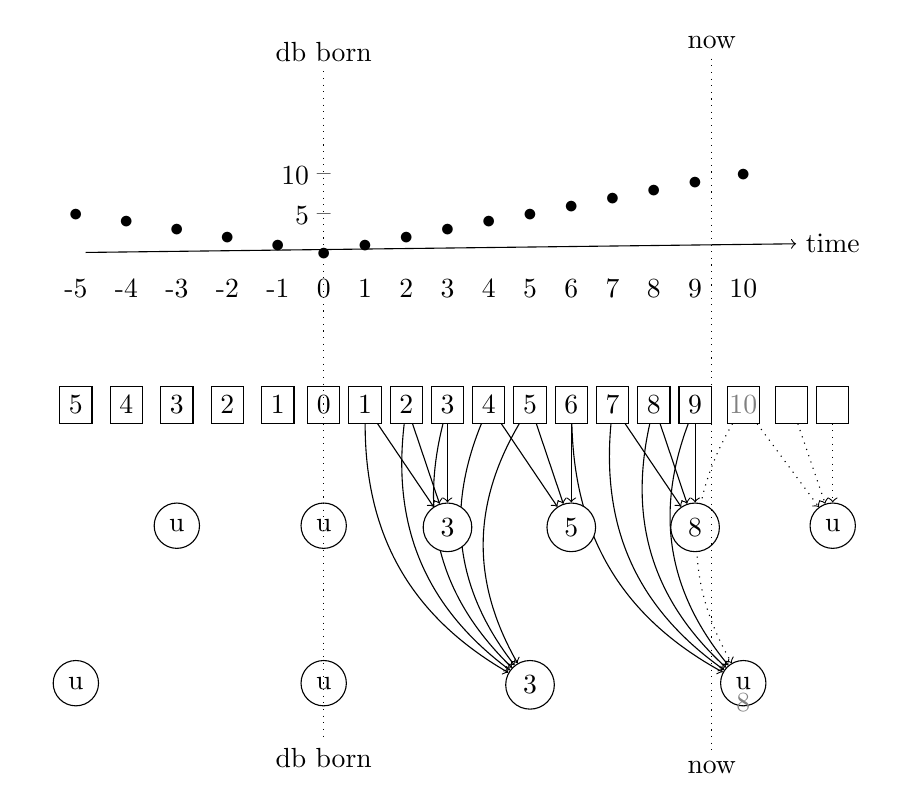
\begin{tikzpicture}

  %referencia
  \node (-6) {};

  \foreach \x in {-5,...,12}
  {
    \pgfkeys{/pgf/number format/.cd,int trunc}
    \pgfmathparse{abs(\x)}
    \let\absx=\pgfmathresult
    \pgfmathparse{\x-1}
    \let\antx=\pgfmathresult
    %time
    \node[node distance=1mm] (\x) [right=of \antx] 
    {\ifnum\x<11 \x \else \phantom{9} \fi};

    %graph values
    \node [above=\absx mm of \x] 
    {\ifnum\x<11 $\bullet$ \fi};    

    %values
    \node[rectangle,draw] (s\x) [below=of \x] 
    {\ifnum\x<10 \pgfmathprintnumber{\absx} \else \phantom{9} \fi};
  }

  \node [below=of 10] {\color{gray}10}; 
  

  
  %rd: 5s |inf| mean
  \node [circle,draw] (rd5-5) [below=3cm of s-5] {u};
  \node [circle,draw] (rd50) [below=3cm of s0] {u};
  \node [circle,draw] (rd55) [below=3cm of s5] {3};
  \node [circle,draw] (rd510) [below=3cm of s10] {u};
  \node [below=3.3cm of s10] {\color{gray}8};
 
  \draw[->,bend right] (s5) to (rd55);
  \draw[->,bend right] (s4) to (rd55);
  \draw[->,bend right] (s3) to (rd55);
  \draw[->,bend right] (s2) to (rd55);
  \draw[->,bend right] (s1) to (rd55);

  \draw[->,dotted,bend right] (s10) to (rd510);
  \draw[->,bend right] (s9) to (rd510);
  \draw[->,bend right] (s8) to (rd510);
  \draw[->,bend right] (s7) to (rd510);
  \draw[->,bend right] (s6) to (rd510);

  
  %rd: 3s |inf| mean
  \node [circle,draw] (rd3-3) [below=of s-3] {u};
  \node [circle,draw] (rd30) [below=of s0] {u};
  \node [circle,draw,fill=white] (rd33) [below=of s3] {3};
  \node [circle,draw,fill=white] (rd36) [below=of s6] {5};
  \node [circle,draw,fill=white] (rd39) [below=of s9] {8};
  \node [circle,draw] (rd312) [below=of s12] {u};

  \draw[->] (s3) to (rd33);
  \draw[->] (s2) to (rd33);
  \draw[->] (s1) to (rd33);

  \draw[->] (s6) to (rd36);
  \draw[->] (s5) to (rd36);
  \draw[->] (s4) to (rd36);

  \draw[->] (s9) to (rd39);
  \draw[->] (s8) to (rd39);
  \draw[->] (s7) to (rd39);

  \draw[->,dotted] (s12) to (rd312);
  \draw[->,dotted] (s11) to (rd312);
  \draw[->,dotted] (s10) to (rd312);



  %eixos
  \node (et0) [above=1mm of -5] {};
  \node (et12) [above=1mm of 12] {time};
  \draw[->] (et0) to (et12);
  \node (y5) [above=5mm of 0] {--};
  \node [left=-1.5mm of y5] {5};
  \node (y10) [above=10mm of 0] {--};
  \node [left=-1.5mm of y10] {10};

  \node (inici) [above=4cm of s0] {db born};
  \node (inici2) [below=4cm of s0] {db born};
  \draw[-,dotted] (inici) to (inici2);

  \node (fi) [above=4.4cm of s9.east] {now};
  \node (fi2) [below=4.4cm of s9.east] {now};
  \draw[-,dotted] (fi) to (fi2);



\end{tikzpicture}



%%% Local Variables:
%%% TeX-master: "../main"
%%% ispell-local-dictionary: "british"
%%% End:
